\chapter{Radargrundlagen}
In diesem Kapitel werden die für diese Arbeit nötigen Grundlagen hergeleitet und erklärt. 
\section{Radar}
Ein Radar versendet eine elektromagnetische Welle und empfängt, falls ein Objekt in Ausbreitungsrichtung vorhanden ist, die davon reflektierte Welle. Aus Unterschieden zwischen beiden Wellen lassen sich verschiedene Informationen, wie Ort und Geschwindigkeit eines Objekts erkennen. Radar\footnote{\textbf{RA}dio \textbf{D}etection \textbf{A}nd \textbf{R}anging} ist dabei die Bezeichnung für diese Form von Erkennungsverfahren und nutzt dabei drei grundlegende physikalische Gesetze von elektromagnetischen Wellen aus:
\begin{description}
\item Definierte Reflexion an Objekten \\
Wenn ein elektrisch leitendes Objekt getroffen wird, kommt es zu einer Reflexion. Diese neue Welle lässt sich mit einem Empfänger erkennen. 
\item Konstante Geschwindigkeit im Freiraum\footnote{Freiraum bezeichnet den mit Luft gefüllten Bereich zwischen Sender und Zielobjekt} \\
Durch konstante Geschwindigkeit lässt sich die über Messung bis zum Erkennen einer reflektierten elektromagnetischen Welle die Entfernung zu einem Objekt bestimmen. 
\item Geradlinige Ausbreitung \\
Durch spezielle Antennen ist es möglich, Winkel zwischen Sender und Objekt zu bestimmen.
\end{description}
Dabei ist der Begriff Radar nur ein Überbegriff für verschiedene Funktionsweisen die die genannten Gesetzmäßigkeiten nutzen. Anschaulich ist das Radarprinzip in Bild dargestellt.

%%BILD FUER HERLEITUNG

Anschaulich ist das Radarprinzip in Bild dargestellt. Dabei muss zwischen einem monostatischem und einem bistatischem Radar unterschieden werden. In einem monostatischem Radar befinden sich Sender und Empfänger am selben Ort. In einem bistatischem Radar ist der Ort unterschiedlich. \\
Um aus Bild einen Zusammenhang zwischen Sende- und Empfangsleistung zu erhalten wird vorrausgesetzt, dass Sender und Empfänger am gleichen Ort sind, es also ein monostatisches Radar ist. Dabei ist die Sendeleistung $P_{S}$ die Leistung der vom Sender erzeugten Welle, die mit dem Antennengewinn $G_{S}$ abgestrahlt wird. Mit Entfernung von Radar zu Objekt $R$ und dem Rückstrahlfläche $\sigma$ wird eine reflektierte Leistung in entgegengesetzter Richtung, also Richtung Radar, vom Objekt abgestrahlt. Die reflektierte Leistung $P_{R}$ ergibt sich demnach zu
\begin{align}
P_{R} = \frac{P_{S} \cdot G_{S} \cdot \sigma}{4\pi \cdot R^2}.
\end{align} Die Empfangsleistung ergibt sich über die reflektierte Leistung und die Antennenwirkfläche $A$ wobei für $A{W}$ gilt mit dem Antennengewinn der Empfangsantenne $G_{e}$\footnote{In diesem Fall ist die Empfangsantenne und die Sendeantenne identisch, allerdings lässt sich die Herleitung verallgemeinern, wofür diese Unterscheidung notwendig ist}. 
\begin{align}
A = \frac{\lambda^2 \cdot G_{e}}{4\pi}.
\end{align}
Dadurch ergibt sich die über die Empfangsleistungsdichte $S_{E}$, wobei 
\begin{align}
S_{E} = \frac{P_{R}}{4\pi \cdot R^2}.
\end{align}
ist, die 
Empfangsleistung $P_{E}$ mit
\begin{align}
P_{E} = S_{E}\cdot A_{W}.
\end{align}
und mit obigen Gleichungen
\begin{align}
P_{E} = \frac{P_{S} \cdot G_{S} \cdot G_{E} \cdot \sigma \cdot \lambda^2}{(4\pi)^3\cdot R^4}
\end{align}
die Radargleichung\footnote{Einzige Einschränkung ist hier, dass Sender und Empfänger die gleiche Entfernung vom Ziel haben müssen. Mit obigen Einschränkungen ist zusätzlich $G_{S} = G_{E}$ wodurch sich die Radargleichung weiter vereinfacht.}.
Durch Umstellung nach $R$ unter Berücksichtigung der minimale Empfangsleistung $P_{E,min}$\footnote{$P_{E,min}$ ist dabei proportional zur Empfängerbandbreite
$B$, der Empfängerrauschzahl $F$ und dem minimalen Signal-zu-Rausch-Verhältnis $SNR_{min}$.} ergibt sich eine maximale Radarreichweite $R_{max}$ mit
\begin{align}
R_{max} = \sqrt[4]{\frac{P_{S} \cdot G_{E}\cdot G_{S} \cdot \lambda^2 \cdot \sigma}{P_{E,min} \cdot (4\pi)^3}}.
\end{align}
Das Verhältnis von ausgesendeter Leistung und empfangener Leistung bezeichnet die Freiraumdämpfung $F$ oder FSPL\footnote{\textbf{F}ree\textbf{S}pace\textbf{P}ath\textbf{L}oss}. Dabei ist
\begin{align}
F = \frac{P_{E}}{P_{S}} = \left(\frac{4\pi \cdot R}{\lambda}\right)^2.
\end{align} 
und mit Lichtgeschwindigkeit c sowie Frequenz f
\begin{align}
c = \lambda \cdot f.
\label{eq:fzulambda}
\end{align}
die Freiraumdämpfung
\begin{align}
F(f,r) = \left(\frac{4\pi \cdot R \cdot f}{c}\right)^2
\end{align}
eine Funktion in Abhängigkeit der Frequenz, und dem Abstand $R$. Diese Frequenz bleibt konstant. Häufig wird $F(f)$ in dB und mit der englischen Bezeichnung bezeichnet, demnach ist
\begin{align}
\text{FPSL(dB)} &= 10\log_{10}\left(\frac{4\pi \cdot R \cdot f}{c}\right)^2 \notag \\
&= 20 \log_{10}\left( R \right) + 20 \log_{10}\left( f \right) - 147,55 .
\end{align}

\section{Radartypen}
Radarsysteme lassen sich in Impuls- und Dauerstrichradarsysteme unterteilen. Das Impulsradar ist hier nicht beschrieben, da es für die weitere Arbeit keine  Verwendung hat. Als Vertreter der Dauerstrichradare wird besonders auf das FMCW Radar eingegangen.

\subsection{Zielentfernung}
Das Radar sendet eine Signal in den Freiraum aus und misst die Zeit, bis das reflektierte Signal detektiert wird. Dieser Zeitunterschied $\Delta t$ gibt mit Hilfe der konstanten Lichtgeschwindigkeit $c$ den Abstand $R$ von Radar zu Objekt über
\begin{align}
R = \frac{c \cdot \Delta t}{2} 
\end{align} 
an. Bezieht man zusätzlich eine konstante Radialgeschwindigkeit des Ziels mit ein, gilt für den Abstand 
\begin{equation}
R(t) = R_{0} - v_{r} \cdot \left( t-t_{0}\right).
\end{equation}
Für den Laufzeitunterschied gilt demnach nach \cite[Gl. 3.1.11]{HuderRadar}
\begin{equation}
\Delta t = \frac{2R}{c_{0}}
		 = \frac{2}{c_{0}}\left(R_{0} - v_{r} \cdot \left( t-t_{0}\right)\right)
\label{eq:AbstandZuDeltaT}
\end{equation}

\subsection{Dauerstrichradar}
Das Dauerstrichradar, auch CW-Radar\footnote{\textbf{C}ontinuous  \textbf{W}ave Radar} sendet im Gegensatz zum Puls-Radar ein kontinuierliches Signal aus. Durch Laufzeitunterschiede des empfangenen und gesendeten Signals lässt sich so der Abstand zu einem Ziel bestimmen. In Abbildung\ref{fig:cwradar} ist das CW-Radar als Blockschaltbild dargestellt.
\begin{figure}[tbp]
  \centering
  \tikzset{%
	% Self defined bulding blocks. 
	% Nevertheless circutikz has implemented filters, couplers and other components since version 0.4, they are mostly implemented as bipoles.
	% The usage of bipoles: \draw (start) to[lowpass/amp/adc,....] (end).
	% The problem is, that if one wants to use arrows, the arrows in bipoles can not be sat manual (fixed in circuitikz source) AND THEY ARE NOT CONSISTENT
	% Also it's quite a mess, which component is a monopole, simple block, bipol, quad/triple etc
	% Following are a few examples on how to define your own blocks. 
	%
	% % % % % % % % % % % % % % % % % % % % % % % % % % % % % % % % % % % % % % % % % % % % % % % % % % % % % % % % % % % % % % % % % % % % %
	% % % % % % % % % % % % % % % % % % % % % % % % % % % % % % % % % % % % % % % % % % % % % % % % % % % % % % % % % % % % % % % % % % % % %
	% % % % % % % % % % % % % % % % % % % % % % % % % % % % % % % % % % % % % % % % % % % % % % % % % % % % % % % % % % % % % % % % % % % % %
	% % % % % % % % % % % % % % % % % % % % % % % % % % % % % % % % % % % % % % % % % % % % % % % % % % % % % % % % % % % % % % % % % % % % %
	%
	% Standard block definition, the width and height is adopted from the circutizk source code, so don't mind the strange values. Also the linewidth is set according to the circutrikz source code.
	block/.style    	= 	{draw, fill=white, thick, rectangle, minimum height = 0.98cm, minimum width = 0.98cm, node distance=2.5cm, line width=1.5pt},
	%
	% Standard circular block
	circleblock/.style	= 	{draw, fill=white, thick, circle, minimum width = 0.98cm,  line width=1.5pt, node distance=2.5cm},
	%
	% Label for circuitikz nodes, as they're reference is in the middle and not on the outer edge of the node....
	circuitikzlabel/.style	=	{label={[label, label distance=0.5cm]#1}},
	%
	%
	%
	% VCO/Oscillator 
	myVCO/.style			= 	{circleblock, path picture={%
		\draw[line width=0.75pt] 	($(path picture bounding box.west)+(0.09cm,0)$) sin ($(path picture bounding box.center)-(0.2cm,-0.2cm)$) cos  (path picture bounding box.center) sin ($(path picture bounding box.center)-(-0.2cm,0.2cm)$) cos ($(path picture bounding box.east)-(0.09cm,0)$);
		}
	},
	% Amplifier, as circuitikz does only provite amplifiers as 2-ports/bipoles
	myAMP/.style		= 	{block, node distance=2.5cm, path picture={%
		\draw[fill=white, line width=0.75pt] ($(path picture bounding box.center)+(0.7em,0)$) -- ($(path picture bounding box.center)-(0.7em,-0.7em)$) -- ($(path picture bounding box.center)-(0.7em,0.7em)$)  -- cycle;
		}
	},
	% Block	
	myBlock/.style    	= 	{draw, fill=white, thick, rectangle, minimum height = 0.98cm, minimum width = 0.98cm, node distance=2.5cm, line width=1.5pt},
	myBigBlock/.style    	= 	{draw, fill=white, thick, rectangle, minimum height = 0.98cm, minimum width = 2.94cm, node distance=2.5cm, line width=1.5pt},	
	% Same for ADC
	myADC/.style 	=	{block, path picture={%
		\draw[line width=0.75pt] 	(path picture bounding box.south west) -- (path picture bounding box.north east);
		\node[] at ($(path picture bounding box.center)+(-.5em,.5em)$) () {D};
		\node[] at ($(path picture bounding box.center)+(.5em,-.5em)$) () {A};
		} 
	},
	% Same for filters
	myLP/.style	=	{block, path picture={%
		%Sine-Waves
		\draw[line width=.75pt] 	($(path picture bounding box.west)+(0.3em,0)$) sin ($(path picture bounding box.center)-(0.50em,-0.3em)$) cos  (path picture bounding box.center) sin ($(path picture bounding box.center)-(-0.50em,0.3em)$) cos ($(path picture bounding box.east)-(0.3em,0)$);
		\draw[line width=0.75pt] 	($(path picture bounding box.west)+(0.3em,-0.65em)$) sin ($(path picture bounding box.center)-(0.50em,0.35em)$) cos  ( $(path picture bounding box.center)-(0,0.65em)$) sin ($(path picture bounding box.center)-(-0.50em,0.95em)$) cos ($(path picture bounding box.east)-(0.3em,0.65em)$);
		\draw[line width=0.75pt] 	($(path picture bounding box.west)+(0.3em,0.65em)$) sin ($(path picture bounding box.center)-(0.50em,-0.95em)$) cos  ( $(path picture bounding box.center)+(0,0.65em)$) sin ($(path picture bounding box.center)-(-0.50em,-0.35em)$) cos ($(path picture bounding box.east)-(0.3em,-0.65em)$);
		% Cancelation
		\draw[line width=0.75pt] 	($(path picture bounding box.center)-(0.2em,0.2em)$) -- (path picture bounding box.center) -- ($(path picture bounding box.center)+(0.2em,0.2em)$) ;
		\draw[line width=0.75pt] 	($(path picture bounding box.center)-(0.2em,-0.45em)$) -- ($(path picture bounding box.center)+(0,0.65em)$) -- ($(path picture bounding box.center)+(0.2em,0.85em)$) ;
		}
	},
}
\begin{tikzpicture}[line width=0.7pt,>=latex,node distance=2.5cm]
	% First: All building blocks are placed relative to the first component
	\draw (0,0)
		node[myVCO, label={above:Signalgenerator}] (oszi) {}
		% As the coupler ports are not in the middle, based on the size (again extraceted from circutikz source code), an yshift is perfomed to have the input on the same height as the output of the oszillator. The xshift is used to place the VCO and ADC on the same y-value after all.
		% Undo the yshift as the output of the coupler is on the same height as the input of the amplifier
		node[myBlock, right of=oszi,  node distance=5cm, label={above:Sender}] (pa) {$P_{S}$}
		% Circulator is rotated that the ports are on the correct position, normally ports are arranged as follows:
		% 
		%				  o------------o
		%						|
		%						o
		node[circulator, below right of=pa, xshift = 3cm, rotate=90,] (circ) {}
		node[antenna, right of = circ] (antenna) {}
		node[myBlock, below left of=circ,  label={below:Empfänger}] (lna) {$P_{E}$}
		% Used redefinition of label, otherwise the label would be overlapping with the mixer shape
		node[mixer, below of=pa,yshift = -1cm  , circuitikzlabel={below:Mischer}] (mixer) {}
		node[myLP, left of=mixer, label={below:Tiefpass}] (lowpass) {}
		node[myADC, left of = lowpass,node distance=2.5cm, label ={below:Signalverarbeitung}](Sig){}		
		;
		
	% Connect everything together
	\draw[->] (oszi) -- node[above]{$u_{S}(t)$}(pa.west);

	%\draw[] (coupler.1) -| ++(-0.5cm,-0.1cm) node[match, rotate=-90, yscale=-1] {};
	\draw[->] (pa.east) -| node[above left]{$u_{S}(t)$}(circ.2);
	\draw[-] (circ.3) -- (antenna);
	\draw[->] (circ.1) |- node[above left]{$u_{E}(t)$}(lna.east);
	\draw[->] (lna.west) -- node[above]{$u_{E}(t)$}(mixer.east);
	\draw[->] (mixer.west)  -- node[above]{$u_{M}(t)$} (lowpass.east);
	\draw[->] (lowpass.west) -- node[above]{$u_{TP}(t)$}(Sig.east);
	\draw[->] (pa.south) -- node[right]{$u_{S}(t)$}(mixer.north);

\end{tikzpicture}

  \caption{CW-Radar Blockdiagramm}
  \label{fig:cwradar}
\end{figure}
Das Sendesignal $u_{S}(t)$ wird versendet. Das empfangene Signal $u_{E}(t)$ gelangt in den Mischer. Im Mischer wird das empfangene Signal mit dem ursprünglichen Signal gemischt. Daraus ergibt sich das Mischsignal $u_{M}(t)$. Das Mischsignal wird in dem nachfolgenden Tiefpass gefiltert. Das daraus entstehende Tiefpasssignal $u_{TP}(t)$ wird weiterverarbeitet und digitalisiert. \\
Ist das Sendesignal $u_{S}(t)$ mit
\begin{align}
u_{S}(t) =  u_{S} \cos\left( \omega_{S}t + \varphi_{S}\right)
\end{align} 
cosinus-förmig mit Phase $\varphi_{S}$ und Winkelgeschwindigkeit $\omega_{S}$ mit 
\begin{align}
\omega_{S} = 2 \pi f_{s}
\end{align}
und das Empfangssignal  $u_{E}(t)$ 
\begin{align}
u_{E}(t) =  u_{E} \cos\left( \omega_{S}\left(t-\Delta t\right) + \varphi_{S}+\varphi_{E}\right) 
\end{align}
ergibt sich im Mischer ein Mischsignal $u_{M}(t)$ mit
\begin{align}
u_{M}(t) = u_{S}(t)\cdot u_{E}(t) = u_{S} u_{E} \cos\left( \omega_{S}t + \varphi_{S}\right)\cdot \cos\left( \omega_{S}\left(t-\Delta t\right) + \varphi_{S}+\varphi_{E}\right).
\end{align}
Wird die trigonometrische Beziehung 
\begin{align}
\cos \alpha \cdot \cos \beta = \frac{1}{2} \left( \cos \left( \alpha + \beta \right) + \cos \left( \alpha - \beta \right) \right)
\end{align}
betrachtet, ergibt sich für das Mischsignal zwei Frequenzen. Zum Einen die Summe der Frequenzen $2\omega_{s}$ zum Anderen die Subtraktion $-\omega_{s}$. Der Tiefpass wird darauf ausgelegt, dass 
\begin{align}
f_{g,TP} = 2f_{s}
\end{align}
gilt.
Es ist nach \cite[S.43,S.44]{HuderRadar} das Tiefpass-Ausgangssignal $u_{TP}(t)$
\begin{align}
u_{TP}(t) = u_{TP} \cos \left( -\omega_{s} \Delta t + \varphi_{Z}\right)
\end{align} und mit Gleichung \ref{eq:AbstandZuDeltaT} ist
\begin{align}
u_{TP}(t) = u _{TP} \cdot \cos \left( \frac{2 \omega_{S} }{c_{0}}\cdot \left( -R_{0} + v_{r}\cdot t - 2 v_{r}\cdot t_{0}\right) +\varphi_{E}\right). 
\end{align}
Ist die Radialgeschwindigkeit $v_{r}$ gleich Null, also keine Bewegung der Sender/Empfängersysteme oder des Ziels, ergibt sich ein konstantes Ausgangssignal am Tiefpass. Dieses konstante Signal lässt sich in die Entfernung zum Ziel umrechnen. 
\subsection{Dauerstrichradar mit Frequenzmodulation}
Das Dauerstrichradar mit Frequenzmodulation, auch FMCW\footnote{\textbf{F}requency \textbf{M}odulated \textbf{C}ontinous \textbf{W}ave}-Radar genannt, beschreibt ein Dauerstrichradar, in welchem das Sendesignal frequenzmoduliert und nicht amplitudenmoduliert wird. Dabei ist der gerätetechnische Aufbau in Abbildung \ref{fig:FMCWRadar} dargestellt. 
\begin{figure}[tbp]
  \centering
  \input{gfx/FMCW_Block_Bjoern.tikz}
  \caption{Blockschaltbild FMCW-Radar}
  \label{fig:FMCWRadar}
\end{figure}
Das aus dem Frequenzmodulator frequenzmodulierte Signal wird über den Sender abgestrahlt. Dabei ergibt sich für das Sendesignal
\begin{align}
u_{s}(t) = u_{s} \cdot \cos\left( 2\pi f_{s}(t) + \varphi_{s} \right) 
\end{align}     
mit Amplitude $u_{s}$ und Phase $\varphi_{s}$. Durch den Frequenzmodulator ergibt sich zusätzlich für die Sendefrequenz $f_{s}(t)$
\begin{align}
f_{s}(t) = f_{0} + \frac{\Delta f}{T_{m}}\cdot t.
\end{align}
\begin{figure}[tbp]
  \centering
  \tikzset{%
	% Self defined bulding blocks. 
	% Nevertheless circutikz has implemented filters, couplers and other components since version 0.4, they are mostly implemented as bipoles.
	% The usage of bipoles: \draw (start) to[lowpass/amp/adc,....] (end).
	% The problem is, that if one wants to use arrows, the arrows in bipoles can not be sat manual (fixed in circuitikz source) AND THEY ARE NOT CONSISTENT
	% Also it's quite a mess, which component is a monopole, simple block, bipol, quad/triple etc
	% Following are a few examples on how to define your own blocks. 
	%
	% % % % % % % % % % % % % % % % % % % % % % % % % % % % % % % % % % % % % % % % % % % % % % % % % % % % % % % % % % % % % % % % % % % % %
	% % % % % % % % % % % % % % % % % % % % % % % % % % % % % % % % % % % % % % % % % % % % % % % % % % % % % % % % % % % % % % % % % % % % %
	% % % % % % % % % % % % % % % % % % % % % % % % % % % % % % % % % % % % % % % % % % % % % % % % % % % % % % % % % % % % % % % % % % % % %
	% % % % % % % % % % % % % % % % % % % % % % % % % % % % % % % % % % % % % % % % % % % % % % % % % % % % % % % % % % % % % % % % % % % % %
	%
	% Standard block definition, the width and height is adopted from the circutizk source code, so don't mind the strange values. Also the linewidth is set according to the circutrikz source code.
	block/.style    	= 	{draw, fill=white, thick, rectangle, minimum height = 0.98cm, minimum width = 0.98cm, node distance=2.5cm, line width=1.5pt},
	%
	% Standard circular block
	circleblock/.style	= 	{draw, fill=white, thick, circle, minimum width = 0.98cm,  line width=1.5pt, node distance=2.5cm},
	%
	% Label for circuitikz nodes, as they're reference is in the middle and not on the outer edge of the node....
	circuitikzlabel/.style	=	{label={[label, label distance=0.5cm]#1}},
	%
	%
	%
	% VCO/Oscillator 
	myVCO/.style			= 	{circleblock, path picture={%
		\draw[line width=0.75pt] 	($(path picture bounding box.west)+(0.09cm,0)$) sin ($(path picture bounding box.center)-(0.2cm,-0.2cm)$) cos  (path picture bounding box.center) sin ($(path picture bounding box.center)-(-0.2cm,0.2cm)$) cos ($(path picture bounding box.east)-(0.09cm,0)$);
		}
	},
	% Amplifier, as circuitikz does only provite amplifiers as 2-ports/bipoles
	myAMP/.style		= 	{block, node distance=2.5cm, path picture={%
		\draw[fill=white, line width=0.75pt] ($(path picture bounding box.center)+(0.7em,0)$) -- ($(path picture bounding box.center)-(0.7em,-0.7em)$) -- ($(path picture bounding box.center)-(0.7em,0.7em)$)  -- cycle;
		}
	},%%
	% Block	
	myBlock/.style    	= 	{draw, fill=white, thick, rectangle, minimum height = 0.98cm, minimum width = 0.98cm, node distance=2.5cm, line width=1.5pt},
	myBigBlock/.style    	= 	{draw, fill=white, thick, rectangle, minimum height = 0.98cm, minimum width = 2.94cm, node distance=2.5cm, line width=1.5pt},	
	% Same for ADC
	myADC/.style 	=	{block, path picture={%
		\draw[line width=0.75pt] 	(path picture bounding box.south west) -- (path picture bounding box.north east);
		\node[] at ($(path picture bounding box.center)+(-.5em,.5em)$) () {D};
		\node[] at ($(path picture bounding box.center)+(.5em,-.5em)$) () {A};
		} 
	},
	% Same for filters
	myLP/.style	=	{block, path picture={%
		%Sine-Waves
		\draw[line width=.75pt] 	($(path picture bounding box.west)+(0.3em,0)$) sin ($(path picture bounding box.center)-(0.50em,-0.3em)$) cos  (path picture bounding box.center) sin ($(path picture bounding box.center)-(-0.50em,0.3em)$) cos ($(path picture bounding box.east)-(0.3em,0)$);
		\draw[line width=0.75pt] 	($(path picture bounding box.west)+(0.3em,-0.65em)$) sin ($(path picture bounding box.center)-(0.50em,0.35em)$) cos  ( $(path picture bounding box.center)-(0,0.65em)$) sin ($(path picture bounding box.center)-(-0.50em,0.95em)$) cos ($(path picture bounding box.east)-(0.3em,0.65em)$);
		\draw[line width=0.75pt] 	($(path picture bounding box.west)+(0.3em,0.65em)$) sin ($(path picture bounding box.center)-(0.50em,-0.95em)$) cos  ( $(path picture bounding box.center)+(0,0.65em)$) sin ($(path picture bounding box.center)-(-0.50em,-0.35em)$) cos ($(path picture bounding box.east)-(0.3em,-0.65em)$);
		% Cancelation
		\draw[line width=0.75pt] 	($(path picture bounding box.center)-(0.2em,0.2em)$) -- (path picture bounding box.center) -- ($(path picture bounding box.center)+(0.2em,0.2em)$) ;
		\draw[line width=0.75pt] 	($(path picture bounding box.center)-(0.2em,-0.45em)$) -- ($(path picture bounding box.center)+(0,0.65em)$) -- ($(path picture bounding box.center)+(0.2em,0.85em)$) ;
		}
	},
}
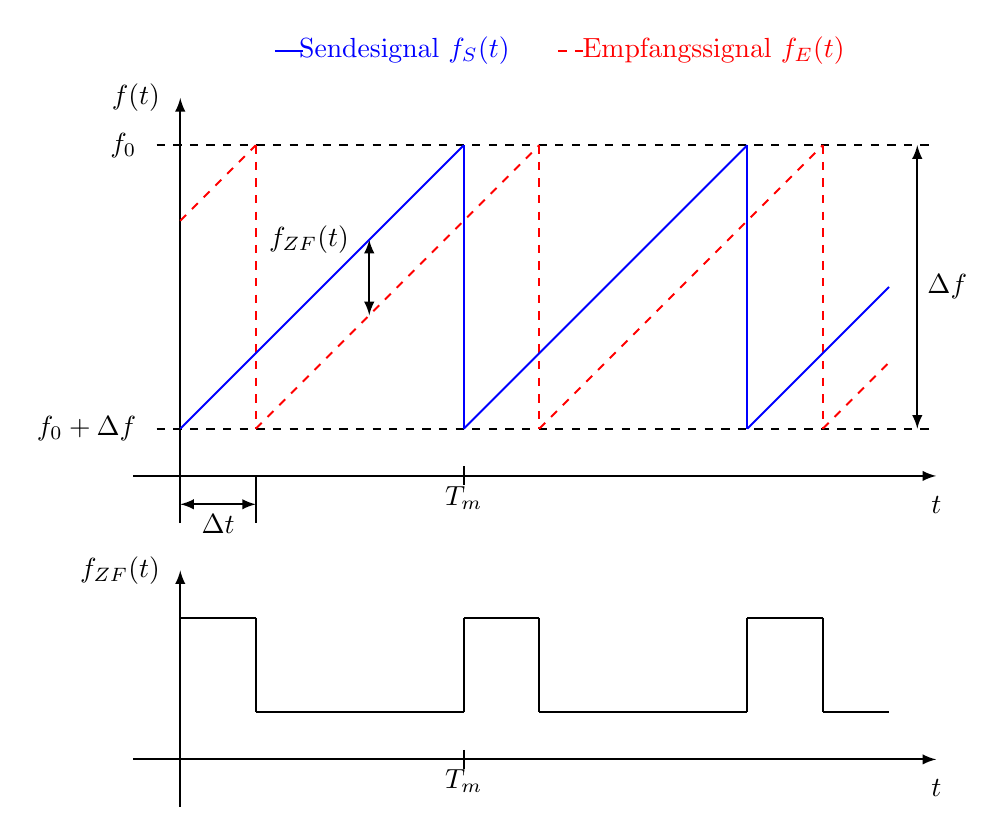
\begin{tikzpicture}[line width=0.7pt,>=latex,node distance=2.5cm,scale = 1.2]

	%Achsen oben
	\draw[->] (-0.5,0) -- (8,0);
	\draw[->] (0,-0.5) -- (0,4); 
	\draw(8,0) node[label={below: $t$}](){};
	\draw(0,4) node[label={left: $f(t)$}](){};
	
	%Achsen unten
	\draw[->] (-0.5,-3)--(8,-3);
	\draw(0,-1) node[label={left: $f_{\text{ZF}}(t)$}](){};
	\draw[->] (0,-3.5)--(0,-1);
	\draw(8,-3) node[label={below: $t$}](){};
	
	%Dashed oben
	\draw[dashed](-0.25,3.5) --(8,3.5);
	\draw(-0.25,3.5) node[label={left: $f_{0}$}](){};
	\draw[dashed](-0.25,0.5) --(8,0.5);
	\draw(-0.25,0.5) node[label={left: $f_{0} + \Delta f$}](){};
	
	%Label Bereich Delta t
	\draw[-] (0.8,0)--(0.8,-0.5);
	\draw[<->](0,-0.3) -- node[below]{$\Delta t$}(0.8,-0.3);
	
	%Label Rechts Delta f 
	\draw[<->](7.8,0.5)--node[right]{$\Delta f$}(7.8,3.5);
	
	%fzf
	\draw[<->](2,1.7)--(2,2.5);
	\draw (2,2.5) node[label ={ left :$f_{\text{ZF}}(t)$}](){};

	%Schwarz unten
	\draw[-] (0,-1.5) -- (0.8,-1.5);
	\draw[-] (0.8,-1.5) -- (0.8,-2.5);
	\draw[-] (0.8,-2.5) -- (3,-2.5);
	\draw[-] (3,-2.5) -- (3,-1.5);
	\draw[-] (3,-1.5) -- (3.8,-1.5);
	\draw[-] (3.8,-1.5) --(3.8,-2.5);
	\draw[-] (3.8,-2.5) --(6,-2.5);
	\draw[-] (6,-2.5) -- (6,-1.5);
	\draw[-] (6,-1.5) --(6.8,-1.5);
	\draw[-] (6.8,-1.5) --(6.8,-2.5);
	\draw[-] (6.8,-2.5) --(7.5,-2.5);
		
	%Dashed Rot
	\draw[dashed,red](0,2.7) -- (0.8,3.5);
	\draw[dashed,red](0.8,3.5) -- (0.8,0.5);
	\draw[dashed,red](0.8,0.5) -- (3.8,3.5);
	\draw[dashed,red](3.8,3.5) -- (3.8,0.5);
	\draw[dashed,red](3.8,0.5) -- (6.8,3.5);
	\draw[dashed,red](6.8,3.5) -- (6.8,0.5);
	\draw[dashed,red](6.8,0.5) -- (7.5,1.2);
	
	% Blau
	\draw[-,blue](0,0.5)--(3,3.5);
	\draw[-,blue](3,3.5)--(3,0.5);
	\draw[-,blue](3,0.5)--(6,3.5);
	\draw[-,blue](6,3.5)--(6,0.5);
	\draw[-,blue](6,0.5)--(7.5,2);
	
	%Achsen Tm
	\draw[-](3,0.1)--node[below]{$T_{m}$}(3,-0.1);
	\draw[-](3,-2.9)--node[below]{$T_{m}$}(3,-3.1);	
	
	%Legende
	\draw[blue,-] (1,4.5)--node[right]{Sendesignal $f_{\text{S}}(t)$}(1.3,4.5);
	\draw[red,dashed] (4,4.5)--node[right]{Empfangssignal $f_{\text{E}}(t)$}(4.3,4.5);
\end{tikzpicture}

  \caption{Frequenzverlauf Sende-,  Empfangs-und Zwischenfrequenzsignal\cite[S.6]{Huegler}\cite[S.78]{HuderRadar}}
  \label{fig:FMCW_Frequenz}
\end{figure}
Dabei sind in Abbildung\ref{fig:FMCW_Frequenz} der Frequenzhub $\Delta f$, die Modulationsperiode $T_{m}$ sowie der Frequenzoffset $f_{0}$ dargestellt. Der Frequenzverlauf ist hier als sägezahnförmig angenommen. Andere Formen, beispielsweise sinuförmig oder linear, sind ebenfalls möglich. Zusätzlich wird auf die erste Modulationsperiode beschränkt. Für weitere Perioden gilt das Vorgehen analog.\\
Das Empfangssignal $s_{e}(t)$ wird um den Laufzeitunterschied $\Delta t$ mit
\begin{align}
\Delta t = \frac{2R}{c_{0}}
\end{align}
verschoben. Dabei ist R der Radar-Ziel Abstand. Dadurch ergibt sich für die Empfangsfrequenz $f_{e}(t)$ 
\begin{align}
f_{e}(t) = f_{0} + \frac{\Delta f}{T_{m}}\cdot \left( t-\Delta t \right).
\end{align}
Ist zudem der in Abbildung \ref{fig:FMCWRadar} dargestellte Tiefpass darauf ausgelegt, die Summenfrequenz $f_{s} + f_{e}$ nicht passieren zu lassen, ergibt sich analog zu \cite[S.43,S.44]{HuderRadar} für die Zwischenfrequenz
\begin{align}
f_{ZF}(t) = \vert f_{s}(t)- f{e}(t) \vert = \frac{\Delta f}{T_{m}}\cdot \Delta T.
\end{align}
Damit ist die Zwischenfrequenzspannung $u_{ZF}(t)$ 
\begin{align}
u_{ZF}(t) = u_{ZF} \cdot  \cos\left( 2\pi \frac{\Delta f \Delta t}{T_{m}} \cdot t + \varphi_{s} \right) .
\end{align}
Daraus ergibt sich nach\cite[S.80]{HuderRadar} die Zielentfernung $R$ zu
\begin{equation}
R = \frac{c_{0}T_{m}}{2\Delta f}\cdot f_{ZF}.
\end{equation}
Um $R$ zu bestimmen muss die Zwischenfrequenz gemessen werden. Dafür wird das Zwischenfrequenzsignal verarbeitet und anschließend digitalisiert. Das Spektrum des Digitalsignals kann mit einer FFT\footnote{\textbf{F}ast \textbf{F}ourier \textbf{T}ransformation} berechnet werden. Daraus ergibt sich ein diskretes Spektrum, in dem die Zwischenfrequenz erkennbar ist. Falls mehrere Ziele detektiert werden, lassen sich ebenso mehrere Zwischenfrequenzen erkennen.
\subsection{Chirp-Sequence-Radar}
Ein Nachteil des Dauerstrichradar mit Frequenzmodulation ist, dass es nicht ohne weiteres möglich ist, die Radialgeschwindigkeit zu bestimmen. Dafür kann das Dauerstrichradar mit Frequenzmodulation erweitert werden zu einem Chirp-Sequence-Radar. Dabei werden viele, möglichst kurze Rampen als Frequenzmodulation vorgenommen - die einzelnen Rampen sind demnach möglichst Steil. Das Chirp-Sequence-Radar wird zudem nicht über eine einzelne Rampe ausgewertet, sondern über eine feste Menge an Rampen. Im Spektrum entstehen nun eindeutig voneinander trennbare spektrale Anteile die entweder proportional zum Abstand oder zur Geschwindigkeit sind. Bei ausreichender Steilheit finden sich die Anteile die proportional zum Abstand sind in den oberen Bereichen des Spektrums, entsprechend die Anteile der Geschwindigkeit in unteren Teilen des Spektrums. 